\documentclass[]{article}

% Imported Packages
%------------------------------------------------------------------------------
\usepackage{amssymb}
\usepackage{amstext}
\usepackage{amsthm}
\usepackage{amsmath}
\usepackage{enumerate}
\usepackage{fancyhdr}
\usepackage[margin=1in]{geometry}
\usepackage{graphicx}
\usepackage{extarrows}
\usepackage{setspace}
%------------------------------------------------------------------------------

% Header and Footer
%------------------------------------------------------------------------------
\pagestyle{plain}
\renewcommand\headrulewidth{0.4pt}
\renewcommand\footrulewidth{0.4pt}
%------------------------------------------------------------------------------

% Title Details
%------------------------------------------------------------------------------
\title{Deliverable \#2 Group \#1 T02}
\author{SE 3A04: Software Design II -- Large System Design}
\date{}
%------------------------------------------------------------------------------

% Graphix
%------------------------------------------------------------------------------
\graphicspath{ {figures/} }

% Document
%------------------------------------------------------------------------------
\begin{document}

\maketitle

\section{Introduction}
\label{sec:introduction}
% Begin Section

\subsection{Purpose}
\label{sub:purpose}
% Begin SubSection
The purpose of the document is to provide a high level design for the system architecture and class composition. This document is intended for use by the stakeholders of the project as reference throughout the various stages of the SDLC. The primary stakeholders include Prof. Ridha Khedri, who has commissioned this project as part of Software Engineering course SE3A04 as provided by McMaster University, Tutorial Assistants for SE3A04, who are responsible with oversight and review of the deliverables of the project and members of the development team (ie. authors of the document). Other stakeholders include any future teams of developers and managers, that may maintain the application or use this project application as an open source reference.

% End SubSection

\subsection{System Description}
\label{sub:system_description}
% Begin SubSection
Climatar is a world simulation software system illustrating the long term and short term effects of actions with respect to climate, greenhouse gas levels, economic stability and social relations with the governing bodies in the model world. The model world is based in the Avatar: The Last Airbender universe. Users are given governance of one of the four tribes in the Avatar universe: Air, Water, Fire, and Earth. Based on the state of the world and the regions that compose it, news events will be posed to the user that require action. Depending on their decisions the world will morph around the change and consequences will propagate throughout the simulation. All decisions have consequences associated with them, and the user can only react to events pertaining to their region, removing the omnipotent aspect of control, users must react to the changing world dynamically.
% End SubSection

\subsection{Overview}
\label{sub:overview}
% Begin SubSection
The remainder of the document pertains to the high level system design specifically outlining how the system will be structured as illustrated by the Use Case Diagram, Analysis Class Diagram, the inherent Architecture Design, and Class Responsibilities. The document first outlines the use cases for Climatar. The use cases illustrate the business events pertaining to the system and layout the system functionality. Descriptions of each use case aide in formalizing the system functionality from the view points identified previously in the SRS. From the Use Case Descriptions, a Noun-Verb Analysis was completed to create an Analysis Class Diagram. The Analysis Class Diagram acts as a starting point from which the major classes of the system will be extracted. The following section, Architecture Design, utilizes the information gained from the analysis class diagram to develop a system architecture to layout the system is a way such that each sub system has high cohesion and low coupling. Finally a Class Responsibility Collaboration (CRC) Card is developed for each class to formally outline the responsibilities, and dependencies for a given class.
% End SubSection

\vspace{20mm}

% End Section

\section{Use Case Diagram}
\label{sec:use_case_diagram}
% Begin Section

\begin{figure}[ht!]
\centering
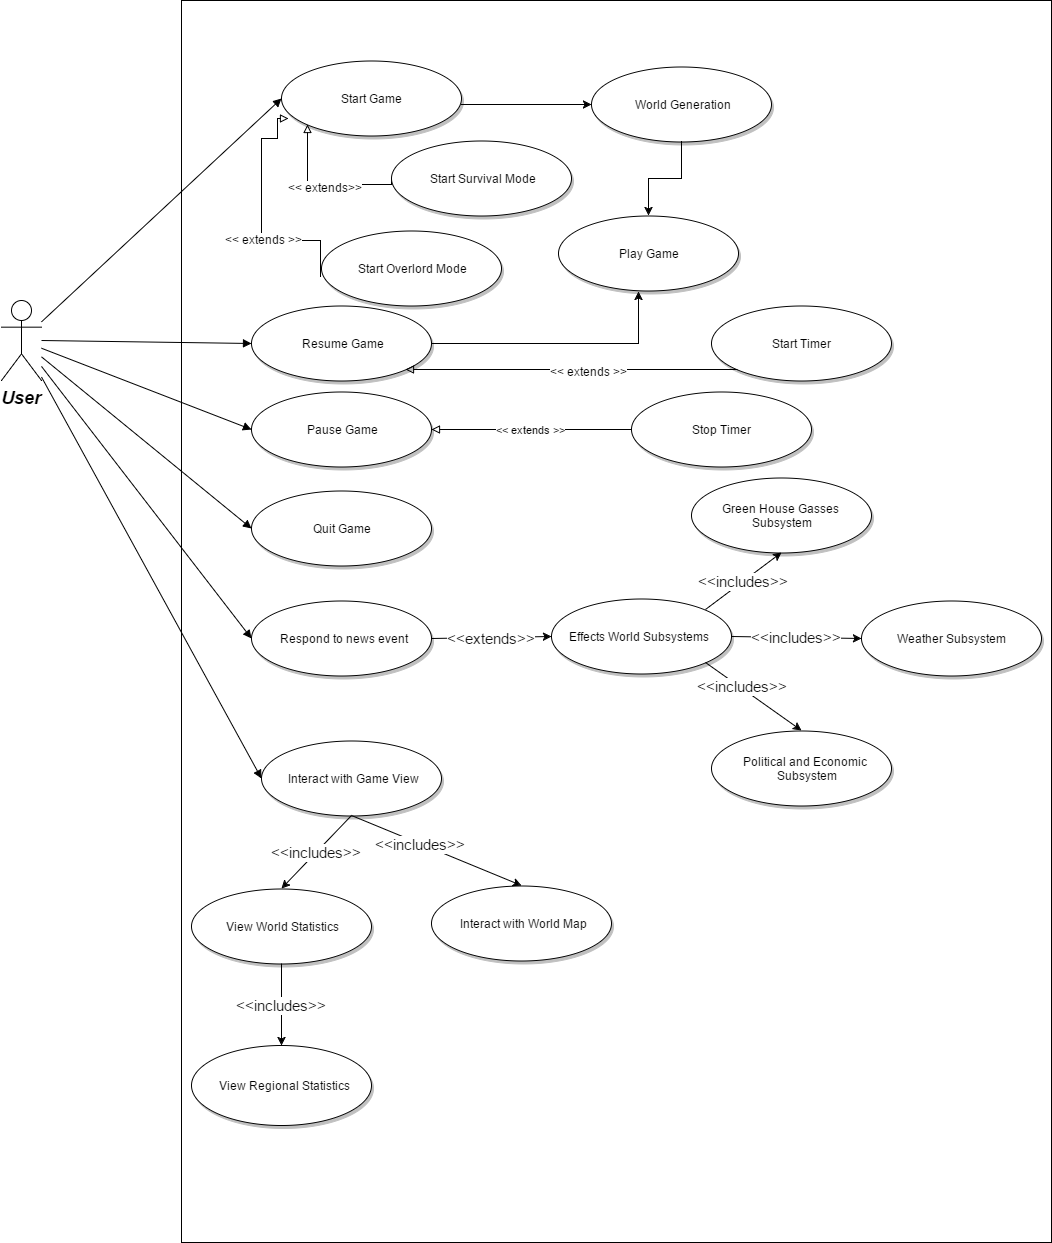
\includegraphics[width=150mm]{ClimatarUseCase}
\caption{Use Case Diagram\label{ucd}}
\end{figure}

\begin{enumerate}[a)]
	\item the main menu screen, the user taps on the start game button which gives the user the option to select the survival game mode or overlord game mode. Selecting one of these options initializes the game world, and switches to the play screen where the user is presented with news events periodically.
\end{enumerate}

\begin{enumerate}[b)]
	\item Selecting one of these game modes, initializes the game world, and switches to the play screen where the user is presented with news events periodically.
\end{enumerate}

\begin{enumerate}[c)]
	\item The user taps the resume button on the play screen which resumes the game system to a playing state.
\end{enumerate}

\begin{enumerate}[d)]
	\item A user taps the pause button to pause the game. The ongoing game transitions to a paused state and timers controlling world simulation the news event generation are paused.
\end{enumerate}

\begin{enumerate}[e)]
	\item A user quits the game. They are prompted if they really want to quit the game early. If they select yes then the current game is destroyed and the game exits to the main menu. Otherwise the game continues unaltered.
\end{enumerate}

\begin{enumerate}[f)]
	\item The user responds to a news event generated by the system, by selecting one of the actions from the news event display. The action is sent back to the game world and it's implications are applied to the subsystems.
\end{enumerate}

\begin{enumerate}[g)]
	\item A user taps the pause button to pause the game. The ongoing game transitions to a paused state and timers controlling world simulation the news event generation are paused.
\end{enumerate}

% End Section

\section{Analysis Class Diagram}
\label{sec:analysis_class_diagram}
% Begin Section

\begin{figure}[ht!]
\centering
\includegraphics[width=140mm]{ClimatarACD}
\caption{Analysis Class Diagram\label{acd}}
\end{figure}

% End Section


\section{Architectural Design}
\label{sec:architectural_design}
% Begin Section
%This section should provide an overview of the overall architectural design of your application. You overall architecture should show the division of the system into subsystems with high cohesion and low coupling.

\subsection{System Architecture}
\label{sub:system_architecture}
% Begin SubSection

The system is divided into the GUI and World subsystems. The World subsystem further divides into Weather, Green House Gases (GHG), Political, and News Event subsystems. The GUI and World sub systems connect to one another but their controls run asynchronously to one another. The selected software architecture for the development of Climatar is Presentation-Abstraction-Control, PAC.

\vspace{3mm}

PAC is the optimal software architecture for Climatar as it helps abstract and modularize the subsystems, allowing also for concurrency between them. Using PAC will also ensure that modules are loosely coupled such that changes do not propagate throughout the system. This principle of loose coupling will make the system more maintainable and extensible in the future. Furthermore, the project has a development time line of approximately one week in which all code will be written. PAC's inherently modular nature allows developers to work in contained subsystems independent of other developers, thus the parallelism for development is optimal.

\begin{figure}[ht!]
\centering
\includegraphics[width=150mm]{ClimatarPACArchitecture}
\caption{System Architecture, PAC\label{pacarch}}
\end{figure}

% End SubSection

\subsection{Subsystems}
\label{sub:subsystems}
% Begin SubSection
The following subsystems compose Climatar:
\begin{itemize}
	\item \textbf{Application:} The Application subsystem is the entry point for the system, and acts as a top level controller for Climatar. This subsystem responds to user stimulus and passes command to the subsystem responsible for handling the stimulus, however this module can only command the World, Menu, and Play subsystems, which compose the control of the remaining subsystems.

	\item \textbf{Play:} The Play subsystem is responsible for displaying all elements composing the games view. Control is passed to this subsystem from Application.

	\item \textbf{Menu:} The Menu subsystem is responsible for all controls and UI components associated with the Main Menu/Title Screen for Climatar, and the game mode the game will be activated in. The Menu is given control by the Application subsystem and can control the FileHandler for loading and saving game instance requests.

	\item \textbf{FileHandler:} The FileHandler subsystem is controlled by the Menu for load and save game requests.

	\item \textbf{World:} The World subsystem is responsible for simulating the world in a Climatar game instance, this includes the information retrieval and interpretation from all world creating subsystems. Regions/Nations are linked to their corresponding subsystems.

	\item \textbf{News:} The News subsystem is responsible for storing possible news events, and responding to news event requests through passing an appropriate event given a specified criteria.

	\item \textbf{Map:} The Map subsystem is responsible for the generation and holding of the current map for a given game instance.

	\item \textbf{Weather:} The Weather subsystem is responsible for the simulation of the weather of a region. This subsystem can be disconnected from the major system and not effect its ability to work, weather will just not be a factor in the simulations.

	\item \textbf{GHG:} The GHG subsystem is responsible for the simulation of the green house gas levels and the rate of change of green house gas levels of a region. This subsystem can be disconnected from the major system and not effect its ability to work, green house gases will just not be a factor in the simulations.

	\item \textbf{Political:} The Political subsystem is responsible for the simulation of the economical aspects of a region and a nations relations with the other nations. This subsystem can be disconnected from the major system and not effect its ability to work, political factors will simply not partake the simulations.

\end{itemize}
A visual representation of the high level system composition can be seen in Figure \ref{usesrelation}.
\begin{figure}[ht!]
\centering
\includegraphics[width=120mm]{ClimatarUsesRelation}
\caption{Module Uses Relation \label{usesrelation}}
\end{figure}
% End SubSection

% End Section

\section{Class Responsibility Collaboration (CRC) Cards}
\label{sec:class_responsibility_collaboration_crc_cards}
% Begin Section
This section should contain all of your CRC cards.

\begin{enumerate}[1.]

	% CRC Card Begin %
	\item
	\begin{tabular}{|p{10cm}|p{4cm}|}
	    \hline
	     \multicolumn{2}{|l|}{\textbf{Class Name:  ApplicationController}} \\
	    \hline
	    \textbf{Responsibility:} & \textbf{Collaborators:} \\
	    \hline
	    Display the menu screen & MenuScreenController \\
	Display the play screen & PlayScreenController \\
	Change the application view & - \\
	Start the world simulator & WorldSimulator \\
	Stop the world simulator & WorldSimulator \\

	    \hline
	  \end{tabular}
	% CRC Card End %

	% CRC Card Begin %
	\item
	\begin{tabular}{|p{10cm}|p{4cm}|}
	    \hline
	     \multicolumn{2}{|l|}{\textbf{Class Name:  ApplicationView}} \\
	    \hline
	    \textbf{Responsibility:} & \textbf{Collaborators:} \\
	    \hline
	    Accept and respond to user inputs and preferences & - \\

	    \hline
	  \end{tabular}
	% CRC Card End %

	% CRC Card Begin %
	\item
	\begin{tabular}{|p{10cm}|p{4cm}|}
	    \hline
	     \multicolumn{2}{|l|}{\textbf{Class Name:  FileHandlerController}} \\
	    \hline
	    \textbf{Responsibility:} & \textbf{Collaborators:} \\
	    \hline
	    Maps a game’s state into text format & - \\
	Saves a game file to the hardware’s persistent storage. & - \\
	Reads a game file from the hardware’s persistent storage. & - \\
	Maps a game file’s text data to a game state. & - \\
	Displays a LoadView prompt. & LoadView \\
	Displays a SaveView prompt. & SaveView \\

	    \hline
	  \end{tabular}
	% CRC Card End %

	% CRC Card Begin %
	\item
	\begin{tabular}{|p{10cm}|p{4cm}|}
	    \hline
	     \multicolumn{2}{|l|}{\textbf{Class Name:  LoadView}} \\
	    \hline
	    \textbf{Responsibility:} & \textbf{Collaborators:} \\
	    \hline
	    Displays a list of save game files. & - \\
	Allows selection of a save game file. & - \\
	Displays a success indicator. & - \\

	    \hline
	  \end{tabular}
	% CRC Card End %

	% CRC Card Begin %
	\item
	\begin{tabular}{|p{10cm}|p{4cm}|}
	    \hline
	     \multicolumn{2}{|l|}{\textbf{Class Name:  SaveView}} \\
	    \hline
	    \textbf{Responsibility:} & \textbf{Collaborators:} \\
	    \hline
	    Displays a success indicator. & - \\

	    \hline
	  \end{tabular}
	% CRC Card End %

	% CRC Card Begin %
	\item
	\begin{tabular}{|p{10cm}|p{4cm}|}
	    \hline
	     \multicolumn{2}{|l|}{\textbf{Class Name:  GHGSystemController}} \\
	    \hline
	    \textbf{Responsibility:} & \textbf{Collaborators:} \\
	    \hline
	    Modify current GHG levels & GHGSystemModel \\
	Check if GHG levels are within safe levels & GHGSystemModel \\
	Update GHG statistics in simulator & WorldSimulator \\

	    \hline
	  \end{tabular}
	% CRC Card End %

	% CRC Card Begin %
	\item
	\begin{tabular}{|p{10cm}|p{4cm}|}
	    \hline
	     \multicolumn{2}{|l|}{\textbf{Class Name:  GHGSystemModel}} \\
	    \hline
	    \textbf{Responsibility:} & \textbf{Collaborators:} \\
	    \hline
	    Maintain GHG level data & - \\

	    \hline
	  \end{tabular}
	% CRC Card End %

	% CRC Card Begin %
	\item
	\begin{tabular}{|p{10cm}|p{4cm}|}
	    \hline
	     \multicolumn{2}{|l|}{\textbf{Class Name:  GHGSystemView}} \\
	    \hline
	    \textbf{Responsibility:} & \textbf{Collaborators:} \\
	    \hline
	    Display GHG statistical data & - \\

	    \hline
	  \end{tabular}
	% CRC Card End %

	% CRC Card Begin %
	\item
	\begin{tabular}{|p{10cm}|p{4cm}|}
	    \hline
	     \multicolumn{2}{|l|}{\textbf{Class Name:  MapView}} \\
	    \hline
	    \textbf{Responsibility:} & \textbf{Collaborators:} \\
	    \hline
	    Retrieves user interaction with World Map & Play Screen Co ntroller \\
	Display map & - \\

	    \hline
	  \end{tabular}
	% CRC Card End %

	% CRC Card Begin %
	\item
	\begin{tabular}{|p{10cm}|p{4cm}|}
	    \hline
	     \multicolumn{2}{|l|}{\textbf{Class Name:  MapGenerator}} \\
	    \hline
	    \textbf{Responsibility:} & \textbf{Collaborators:} \\
	    \hline
	    Can generate a new game world. & - \\
	Uses a MapGenerationModel to procedurally generate a game world. & MapGenerationModel \\

	    \hline
	  \end{tabular}
	% CRC Card End %

	% CRC Card Begin %
	\item
	\begin{tabular}{|p{10cm}|p{4cm}|}
	    \hline
	     \multicolumn{2}{|l|}{\textbf{Class Name:  MapGenerationModel}} \\
	    \hline
	    \textbf{Responsibility:} & \textbf{Collaborators:} \\
	    \hline
	    Knows parameters that alter how a game world is generated. & - \\

	    \hline
	  \end{tabular}
	% CRC Card End %

	% CRC Card Begin %
	\item
	\begin{tabular}{|p{10cm}|p{4cm}|}
	    \hline
	     \multicolumn{2}{|l|}{\textbf{Class Name:  MenuScreen}} \\
	    \hline
	    \textbf{Responsibility:} & \textbf{Collaborators:} \\
	    \hline
	    Accepts and responds to Resume Game Request & MenuScreenController \\
	Accepts and responds to Mute music request & MenuScreenController \\
	Accepts and responds to Mute sounds request & MenuScreenController \\

	    \hline
	  \end{tabular}
	% CRC Card End %

	% CRC Card Begin %
	\item
	\begin{tabular}{|p{10cm}|p{4cm}|}
	    \hline
	     \multicolumn{2}{|l|}{\textbf{Class Name:  MenuScreenController}} \\
	    \hline
	    \textbf{Responsibility:} & \textbf{Collaborators:} \\
	    \hline
	    Opens the menu screen & MenuScreen \\
	Closes the menu screen & MenuScreen \\
	Mutes and unmutes sound & ApplicationController \\
	Mutes and unmutes music & ApplicationController \\
	Set game mode & GameMode \\
	Display game mode selection view & GameModeSelectView \\
	Accepts and responds to Save Game request & FileHandlerControler \\
	Accepts and responds to New Game request & - \\
	Accepts and responds to Load Game Request & FileHandlerControler \\
	Accepts and responds to Quit Game Request & - \\

	    \hline
	  \end{tabular}
	% CRC Card End %

	% CRC Card Begin %
	\item
	\begin{tabular}{|p{10cm}|p{4cm}|}
	    \hline
	     \multicolumn{2}{|l|}{\textbf{Class Name:  GameMode}} \\
	    \hline
	    \textbf{Responsibility:} & \textbf{Collaborators:} \\
	    \hline
	    Receive user’s mode selection & MenuScreenController \\
	Store current mode selection & - \\
	Send constraint for user base on the mode to the MenuScreenController & MenuScreenController \\

	    \hline
	  \end{tabular}
	% CRC Card End %

	% CRC Card Begin %
	\item
	\begin{tabular}{|p{10cm}|p{4cm}|}
	    \hline
	     \multicolumn{2}{|l|}{\textbf{Class Name:  GameModeSelectView}} \\
	    \hline
	    \textbf{Responsibility:} & \textbf{Collaborators:} \\
	    \hline
	    Accept and respond to game mode selection & MenuScreenController \\
	Display game modes & - \\

	    \hline
	  \end{tabular}
	% CRC Card End %

	% CRC Card Begin %
	\item
	\begin{tabular}{|p{10cm}|p{4cm}|}
	    \hline
	     \multicolumn{2}{|l|}{\textbf{Class Name:  NewsEventControl}} \\
	    \hline
	    \textbf{Responsibility:} & \textbf{Collaborators:} \\
	    \hline
	    Retrievers user interaction with news events & PlayScreenController \\

	    \hline
	  \end{tabular}
	% CRC Card End %

	% CRC Card Begin %
	\item
	\begin{tabular}{|p{10cm}|p{4cm}|}
	    \hline
	     \multicolumn{2}{|l|}{\textbf{Class Name:  NewsEventGenerator}} \\
	    \hline
	    \textbf{Responsibility:} & \textbf{Collaborators:} \\
	    \hline
	    Knows how to generate a news event. & NewsEvent \\
	Can pass a news event to the NewsEventControl to be displayed. & NewsEventControl \\
	Can forward a news events selected action to the WorldSimulator. & WorldSimulator \\

	    \hline
	  \end{tabular}
	% CRC Card End %

	% CRC Card Begin %
	\item
	\begin{tabular}{|p{10cm}|p{4cm}|}
	    \hline
	     \multicolumn{2}{|l|}{\textbf{Class Name:  NewsEvent}} \\
	    \hline
	    \textbf{Responsibility:} & \textbf{Collaborators:} \\
	    \hline
	    Knows the textual description of the news event & - \\
	Knows a set of actions that the user can select in response to the news event. & - \\

	    \hline
	  \end{tabular}
	% CRC Card End %

	% CRC Card Begin %
	\item
	\begin{tabular}{|p{10cm}|p{4cm}|}
	    \hline
	     \multicolumn{2}{|l|}{\textbf{Class Name:  PlayScreen}} \\
	    \hline
	    \textbf{Responsibility:} & \textbf{Collaborators:} \\
	    \hline
	    Displays state of the World & PlayScreenController \\
	Display Menu & PlayScreenController \\
	Displays state of subsystems & PlayScreenController \\
	Displays World Map & PlayScreenController \\
	Accepts and responds to news events requests & - \\
	Accepts and responds to world map requests & - \\
	Accepts and responds to Pause Game Request & - \\

	    \hline
	  \end{tabular}
	% CRC Card End %

	% CRC Card Begin %
	\item
	\begin{tabular}{|p{10cm}|p{4cm}|}
	    \hline
	     \multicolumn{2}{|l|}{\textbf{Class Name:  PlayScreenController}} \\
	    \hline
	    \textbf{Responsibility:} & \textbf{Collaborators:} \\
	    \hline
	    Display GHG, Weather, Political and News statistic data & - \\

	    \hline
	  \end{tabular}
	% CRC Card End %

	% CRC Card Begin %
	\item
	\begin{tabular}{|p{10cm}|p{4cm}|}
	    \hline
	     \multicolumn{2}{|l|}{\textbf{Class Name:  PoliticalSystemController}} \\
	    \hline
	    \textbf{Responsibility:} & \textbf{Collaborators:} \\
	    \hline
	    Modify current political levels & PoliticalSystemModel \\
	Check if political levels are within safe levels & PoliticalSystemModel \\
	Update political statistics in simulator & WorldSimulator \\

	    \hline
	  \end{tabular}
	% CRC Card End %

	% CRC Card Begin %
	\item
	\begin{tabular}{|p{10cm}|p{4cm}|}
	    \hline
	     \multicolumn{2}{|l|}{\textbf{Class Name:  PoliticalSystemModel}} \\
	    \hline
	    \textbf{Responsibility:} & \textbf{Collaborators:} \\
	    \hline
	    Maintain political atmosphere data & - \\

	    \hline
	  \end{tabular}
	% CRC Card End %

	% CRC Card Begin %
	\item
	\begin{tabular}{|p{10cm}|p{4cm}|}
	    \hline
	     \multicolumn{2}{|l|}{\textbf{Class Name:  PoliticalSystemView}} \\
	    \hline
	    \textbf{Responsibility:} & \textbf{Collaborators:} \\
	    \hline
	    Display political statistics data & - \\

	    \hline
	  \end{tabular}
	% CRC Card End %

	% CRC Card Begin %
	\item
	\begin{tabular}{|p{10cm}|p{4cm}|}
	    \hline
	     \multicolumn{2}{|l|}{\textbf{Class Name:  WeatherSystemController}} \\
	    \hline
	    \textbf{Responsibility:} & \textbf{Collaborators:} \\
	    \hline
	    Modify current temperature levels & WeatherSystemModel \\
	Check if temperature levels are within safe levels & WeatherSystemModel \\
	Update Weather statistics in simulator & WorldSimulator \\

	    \hline
	  \end{tabular}
	% CRC Card End %

	% CRC Card Begin %
	\item
	\begin{tabular}{|p{10cm}|p{4cm}|}
	    \hline
	     \multicolumn{2}{|l|}{\textbf{Class Name:  WeatherSystemModel}} \\
	    \hline
	    \textbf{Responsibility:} & \textbf{Collaborators:} \\
	    \hline
	    Maintain temperature level data & - \\

	    \hline
	  \end{tabular}
	% CRC Card End %

	% CRC Card Begin %
	\item
	\begin{tabular}{|p{10cm}|p{4cm}|}
	    \hline
	     \multicolumn{2}{|l|}{\textbf{Class Name:  WeatherSystemView}} \\
	    \hline
	    \textbf{Responsibility:} & \textbf{Collaborators:} \\
	    \hline
	    Display weather/temperature statistics & - \\

	    \hline
	  \end{tabular}
	% CRC Card End %

	% CRC Card Begin %
	\item
	\begin{tabular}{|p{10cm}|p{4cm}|}
	    \hline
	     \multicolumn{2}{|l|}{\textbf{Class Name:  WorldState}} \\
	    \hline
	    \textbf{Responsibility:} & \textbf{Collaborators:} \\
	    \hline
	    Store current world information & - \\
	Send world state information to the WorldSimulator & WorldSimulator \\
	Retrieve calculated world state info from WorldSimulator & WorldSimulator \\

	    \hline
	  \end{tabular}
	% CRC Card End %

	% CRC Card Begin %
	\item
	\begin{tabular}{|p{10cm}|p{4cm}|}
	    \hline
	     \multicolumn{2}{|l|}{\textbf{Class Name:  StateView}} \\
	    \hline
	    \textbf{Responsibility:} & \textbf{Collaborators:} \\
	    \hline
	    Retrievers user interaction with World state & PlayScreenController \\
	Retrieves user interaction with World Subsystems & PlayScreenController \\

	    \hline
	  \end{tabular}
	% CRC Card End %

	% CRC Card Begin %
	\item
	\begin{tabular}{|p{10cm}|p{4cm}|}
	    \hline
	     \multicolumn{2}{|l|}{\textbf{Class Name:  WorldSimulator}} \\
	    \hline
	    \textbf{Responsibility:} & \textbf{Collaborators:} \\
	    \hline
	    Generate news events & WeatherSystemController, GHGSystemController, PoliticalSystemController, NewsSystemController \\

	    \hline
	  \end{tabular}
	% CRC Card End %


\end{enumerate}
% End Section

\appendix
\section{Division of Labour}
\label{sec:division_of_labour}
% Begin Section
Include a Division of Labour sheet which indicates the contributions of each team member. This sheet must be signed by all team members.

\begin{tabular}{ | l | l | }
\hline
	\textbf{Contributor Name} & \textbf{Contributions}  \\
  	\hline
  	Wenbin Yuan & Uses Cases and CRC cards. Revised the document. \\
  	\hline
  	Haris Khan &  CRC cards, initial draft of use cases. \\
  	\hline
  	Riley McGee & Original draft of 1.* and 4.* including figures for Module Uses Relation and Architecture\\
  	\hline
		Vishesh Gulatee & Use Cases, CRC cards, and document revision. \\
  	\hline
  	James Taylor & Analysis Class Diagram, use case diagram refinement. \\
  	\hline
\end{tabular}
\\
\\
By signing below you agree to the work divisions stated above correctly representing all contributions made:


% End Section

\newpage
\section*{IMPORTANT NOTES}
\begin{itemize}
%	\item You do \underline{NOT} need to provide a text explanation of each diagram; the diagram should speak for itself
	\item Please document any non-standard notations that you may have used
	\begin{itemize}
		\item \emph{Rule of Thumb}: if you feel there is any doubt surrounding the meaning of your notations, document them
	\end{itemize}
	\item Some diagrams may be difficult to fit into one page
	\begin{itemize}
		\item It is OK if the text is small but please ensure that it is readable when printed
		\item If you need to break a diagram onto multiple pages, please adopt a system of doing so and thoroughly explain how it can be reconnected from one page to the next; if you are unsure about this, please ask about it
	\end{itemize}
	\item Please submit the latest version of Deliverable 1 with Deliverable 2
	\begin{itemize}
		\item It does not have to be a freshly printed version; the latest marked version is OK
	\end{itemize}
	\item If you do \underline{NOT} have a Division of Labour sheet, your deliverable will \underline{NOT} be marked
\end{itemize}


\end{document}
%------------------------------------------------------------------------------
